\documentclass[12pt]{extarticle}
\usepackage{graphicx}
\usepackage{setspace}
\usepackage{xcolor}
\usepackage[a4paper, total={6in, 8in}]{geometry}
\usepackage{pgfgantt}

\begin{document}

\doublespacing

\title{\textbf{Debugging Problems}}
\author{Patrick Farmer\\ Supervisor: Dr. Jonathan Dukes}
\date{\today}
\maketitle

\begin{figure}[h!]
\centering

\includegraphics[width=\linewidth]{Images/Trinity_Main_Logo.jpg}
\label{fig:logo}
\end{figure}

\begin{center}
\large A Dissertation submitted in partial fulfillment of the requirements for the degree of MAI in Computer Engineering.
\end{center}

\newpage
\title {\Huge \textbf{\textcolor{blue}{Declaration}}}

\vspace{0.5cm}
\small I hereby declare that this Dissertation is entirely my own work and that it has not been submitted as an exercise for a degree at this or any other university.

\vspace{0.5cm}
\small I have read and I understand the plagiarism provisions in the General Regulations of the University Calendar for the current year, found at http://www.tcd.ie/calendar.
\vspace{0.5cm}

\small I have completed the Online Tutorial on avoiding plagiarism `Ready Steady Write', located at http://tcd-ie.libguides.com/plagiarism/ready-steady-write.
\vspace{0.5cm}

\small I consent to the examiner retaining a copy of the thesis beyond the examining period, should they so wish (EU GDPR May 2018).
\vspace{0.5cm}

\small I agree that this Dissertation will not be publicly available, but will be available to TCD staff and students in the University’s open access institutional repository on the Trinity domain only, subject to Irish Copyright Legislation and Trinity College Library conditions of use and acknowledgement.
\vspace{2cm}

\small Signed:~Patrick Farmer\hfill Date:~\today

\newpage
\tableofcontents

\newpage
\section{Acronyms}

\begin{itemize}
    \item LLM - Language Model
    \item AST - Abstract Syntax Tree
    \item AI - Artificial Intelligence
    \item API - Application Programming Interface
    \item GPT - Generative Pre-trained Transformer
\end{itemize}
\newpage
\section{Introduction}

\subsection{Context}

In recent years there have been great strides made in the ability of LLMs to generate code. These LLMs are already being integrated into employee workflows in companies all over the world. This will place a much greater emphasis on the debugging process as the code generated by these LLMs much be inspected and fixed when bugs are produced. It has also been noted in many studies that debugging is an extremely important skill as it is the most difficult part of the programming process and is also the most often overlooked when teaching programming. More will be discussed on this in the literature review. This project will aim to create a tool that will help teach debugging to students who will be the future employees of these companies. 

\subsection{Aims}

The aim of this tool is quite simple. To generate problems for students. The language, code topic and bug type should all be customisable. 

It was also a goal to create two different methods for inserting the bug which can be compared with each other. The first method being to insert the bug by querying the LLM and the second method being to insert the bug by walking through the AST of the code and inserting the bug semi manually.

Another aim of the project was to create test cases that the code could be tested against to ensure that the bug was inserted correctly. These same test cases could then be used by a student to test their solution to the problem.

The creation of a frontend was not a goal of this project, the meaningful work of this project is all done in the backend and a frontend could be added at a later date.

\subsection{Evaluation Metrics}

It was decided early on that the evaluation and measuring of the project success would be done using desktop metrics and that there would not be a user study. The metrics that were decided on were code complexity, code diversity, attempt count and run time. The calculation of these metrics and the reasoning behind them will be discussed in the testing and evaluation section.

\subsection{Structure of the Dissertation}

The structure of the dissertation will be as follows. The background will go through previous work done in the area of debugging and LLMS. It will also give a brief overview of how LLMs work and more importantly how they can be used to generate code, the difficulties that come with using them and where they excel. 

The design and implementation will show how the code is structured and will give a brief description of how each part of the code works.

The testing and evaluation section will show the testing that was done on the project and the results of that testing. It will also discuss the metrics used in testing, why they were chosen and how they were calculated.

The conclusion will summarise the project and discuss the future of the project.
\newpage
\section{Background}

\subsection{Literature Review}

Debugging has always been an essential aspect of programming, yet many universities do not teach it specifically. This is highlighted by Li in \cite{li2019}. As previously mentioned, the significance of debugging skills has grown markedly now that AI is becoming more prevalent in industry, as noted by Denny in \cite{denny2024}. Debugging itself includes several sub-domains, as outlined in \cite{li2019} as language knowledge, understanding of the specific program, and skill in the debugging process. This project primarily focuses on developing the debugging skill but there will be some domain knowledge that comes with it.\\
\\
When novice programmers write code, they inevitably introduce bugs, but as Jadud mentions in \cite{jadud2006}, they often respond by making minor syntax tweaks and rerunning their code immediately rather than trying to identify and resolve the underlying issue. This is another challenge that this tool addresses: by inserting deeper bugs, students are compelled to scrutinize and understand the code.\\
\\
Another important aspect of debugging that this tool addresses is the use of debugging tools like Python’s debugger, which are part of the sub-domains indicated by Li in \cite{li2019}. Learning to effectively use these debuggers can considerably improve students’ debugging abilities. However, Odell \cite{odell2017} argues that forcing students to think about the program without any tool-assisted help is the most effective instructional approach. Ultimately, each professor can decide whether to allow debugging tools, depending on the objectives of their particular assignment.\\
\\
As Nguyen states in \cite{nguyen2024}, significant misunderstandings can easily arise between an AI and its user, which is especially true for novices who may struggle to articulate their problems thoroughly. This situation creates a chance to teach students how to harness LLMs effectively. The future frontend may benefit from incorporating a co-pilot like assistance, allowing professors to enable or disable it depending on the complexity level they want to set. A comparable methodology is described by Denny in \cite{denny2023}, where students restricted to using LLMs alone learned to refine their prompts for more accurate output.

\subsection{Summary of LLMs}
\subsubsection{How LLMs work}

LLMs in essentials are a type of neural network that is trained on a large dataset of text and commonly code. They are trained to predict the next token in a sentence. The common chat bots works by rephrasing your input and allowing the LLM to predict the next token which when it continues will create a response to your question or prompt.

\subsubsection{Using LLMs}

For interacting with an LLM you will generally use an API. This tool uses two different APIs to interact with LLMs which can be swapped inbetween. The first API is the OpenAI GPT API which is a paid API that is very accurate and very fast, in an ideal world this would be used for all versions and iterations for the project. However, this is of course going to get very expensive very quickly. For this reason a second method of interacting with local LLMs is used to. This method is much slower and can be less accurate to varying degrees depending on the model but is free except for the small electricity cost and hardware wear and tear. The local LLMs are also more customisable with adjustable hyperparameters and can be fine-tuned on custom datasets, although this was not necessary for this project. A variety of models using the ollama API were used for the vast majority of the project but for final evaluation the same code was run using the OpenAI GPT API for comparison.

\subsubsection{Evaluation of LLMs}

Using an LLM as discussed above is very easy. You simply give the LLM the prompt and read the output. However, there are some difficulties especially with the local LLM. Although the reponses were generally good, they could not simply be taken to be in the expected format. LLMs often provide a response not in the desired format, for that reason there is a lot of code which is used to clean up and parse the response from the LLM. This also leads to the issue of sometimes the LLM will hallucinate and provide an incorrect response, this is the reason for the implementation of self reflection and improvement in the code generation which will be discussed further in the design and implementation section. However, the simple and very significant benefit of using an LLM is that it can generate code with very little effort which makes it the only option for the generation of code for this project.

\newpage
\section{Design and Implementation}

\subsection{Design Overview}
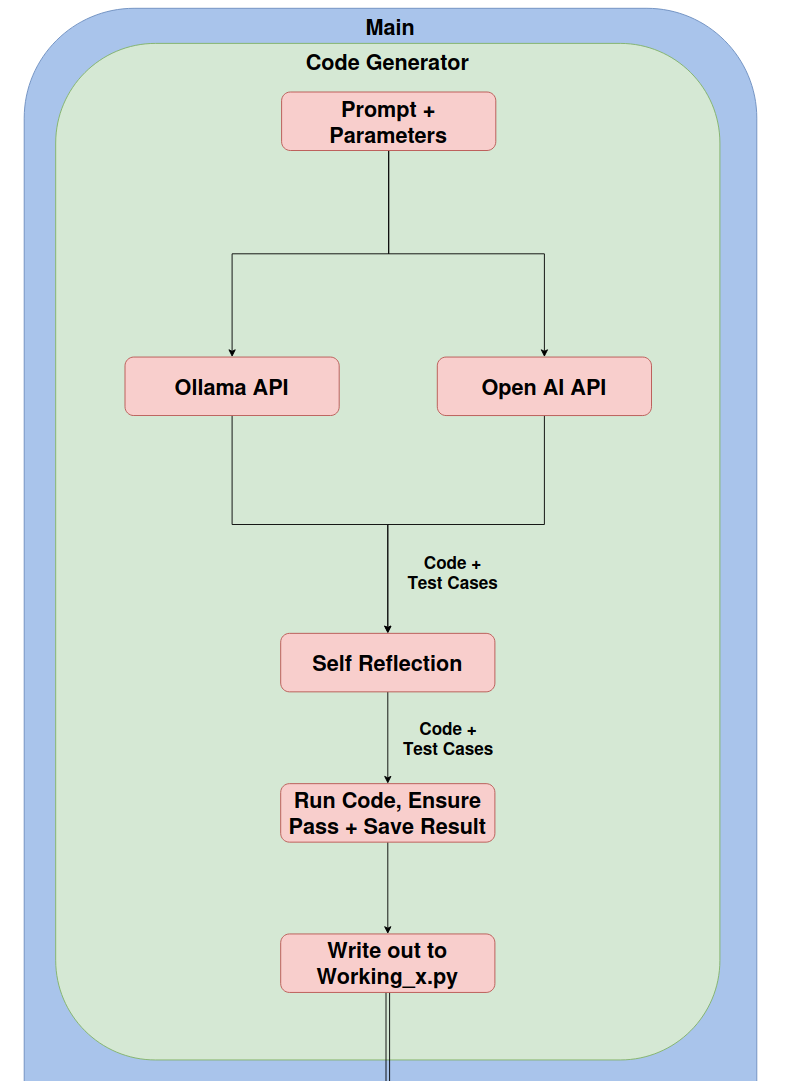
\includegraphics[width=\linewidth]{Images/Tall_design_1.png}

\newpage
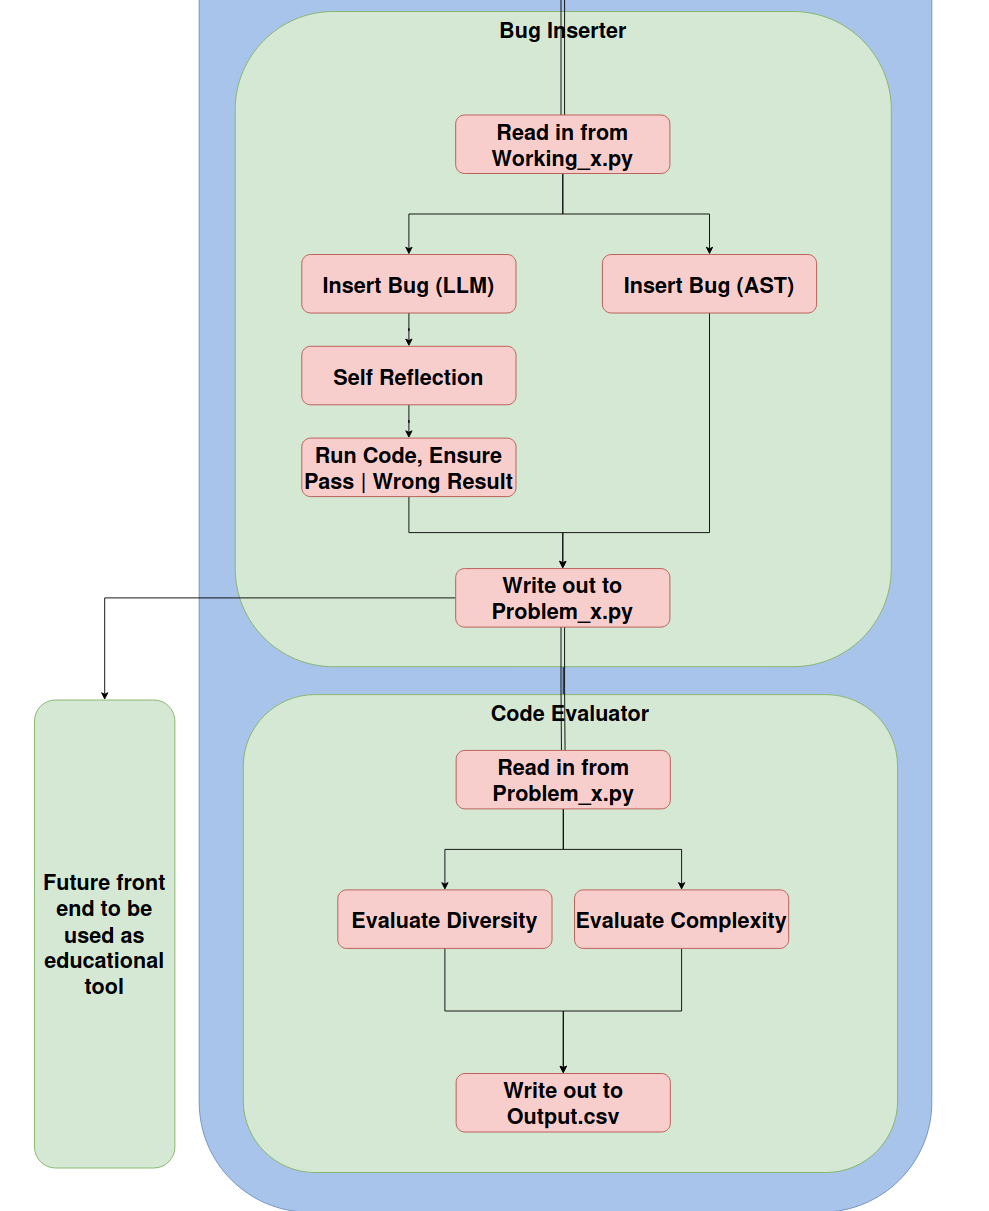
\includegraphics[width=\linewidth]{Images/Tall_design_2.png}

The above diagram shows a pipeline diagram of the code. There is three main blocks to the code. The code generator which takes no input except for simple parameters such as model type and code topic. It will then produce functional code based on the topic mentioned. It will also ensure that the code is functional by compiling and checking for errors. 

The bug inserter will then take this working code and insert a bug into it, this is done by either the use of the LLM again or by using inspecting and altering the AST in the code. It will then check if the code now fails or produces the wrong output as it should do. This is only done for the LLM however as the AST bug inserter is not liable the same reliability issues of the LLM. This altered code is then written back out to the file overwriting the original code. The code evaluator will then take this code and run the diversity and complexity metrics on it before writing this to the csv.

\subsection{Tools}
\subsubsection{Ollama}

The first of the two major tools that was used in this project is ollama. This is a tool that facilitates easy interaction with LLMs running on a local machine. This tool allows for the usage of almost all popular models. This tool was downloaded by cloning the ollama repository from github and running the install script. Further models could then easily be pulled and run from command line using the following commands.

\begin{verbatim}
ollama pull <model>
ollama run <model>
<Interaction with LLM>
\end{verbatim}

This works perfectly well for interacting with the LLM like a chat bot but like this through some shell scripting language such as bash would not be the ideal solution. Fortunately the ollama API is much better suited to this task. The constructor for the class is called with some intialising hyperparameters and then a prompt can simple be passes to using the invoke method which returns the response from the LLM. This was then wrapped in a class for easy use in the project.

\subsubsection{OpenAI GPT API}

The process for using the OpenAI GPT API is a bit simpler since there is no setup but has a few more steps in the code for the protection of the API key. Due to this code being on a github repo and automated testing being done using github workflows there is a couple different environments that all need access to the API key. For the github workflow runner the key was stored as a secret and then passed to the code as an environment variable. For the local machine the key was stored in a file which was excluded from git commits using the .gitignore file. One this has been handled the interaction is very similar. The parameters, prompt and API key are passed to the constructor and then a function is called to get the response from the LLM.

\subsection{Code generation}

The code generation class is the first class called in the pipeline and is also the only class that interacts directly with the LLM. The class is called with the model type, file\_path and a number of different switches to enable different modes, the prompt is then adapted and phrased in a way that the code produced will always expect an input file called \texttt{input.txt}. The LLM is then called to generate the code and also generate the \texttt{input.txt} file. Both of these responses are then parsed and written to their respective files. The code is then run from a subprocess which will check if the code compiles and runs correctly. If the code does not compile or run correctly the function will return an error and the parent function will handle it. If it works correctly the function will return the response with the given \texttt{input.txt} which is used to determine later whether the bug inserter has worked correctly. Due to the input being in the format of a separate file it is very easy for multiple \texttt{input.txt} files to be generated and used as multiple different test cases. 
There is also an option for a prompt to be passed to the class which will override the original prompt. This is how the LLM bug insertion is able to interact with the LLM without creating duplicate logic. 

\subsubsection{Self Reflection \& Improvement}

As the project progressed it was clear that the local LLMs were having a lot of difficulty producing the correct code. This was very uncommmon with the openAI modules but to solve this self reflection and improvement was implemented in the code. 

As it became impossible to feed the LLMs more information in training a new technique emerged when developers would get the LLM to 'think' about their response. This is done by re-querying the LLM after it returns a response and asking it if the response it gave fits the original prompt. This process is called self reflection which is good for filtering out bad responses. Another similar method is called self improvement which is where the LLM is asked to improve on its response. This will attempt to fix bad responses and also attempt to improve already acceptable responses.

The issue that was noticed with this method was a significant increase in the runtime of the project. However it also meant that smaller modeuls could be used and provide better performance. It is not clear which method would be likely to yield a better response but the performance will be compared and discussed in the testing and evaluation section.

\subsection{Bug Insertion}
\subsubsection{LLM Bug Insertion}

The first method for bug insertion that was used was the LLM bug inserter. This method is very simple as it uses the same function as the code generation step but with a switch to override the prompt. This will mean it can then very easily run the same test cases and check if the code now fails or produces the wrong output. If the result is the same as before it will be assumed that the bug was either not inserted or does not necessarily change the output. This was a simple addition as there was little additional code to be written but it was also quite unreliable. Although it was in theory completing a much smaller task than the code generation step, it saw a lot more issues with the LLMs hallucinating and providing incorrect responses. This was likely due to the task was a bit less intuitive as there is a lot less information to go on when inserting a bug than when generating code, and as a result less information in the training data and therefore less accurate responses in this case.

\subsubsection{AST Bug Insertion}

The second method for bug insertion was the AST bug inserter. This method was much more reliable and also massively faster. However, it has the disadvantage of being much less customisable than the LLM method. There is two different bug types that can be inserted. There is a syntax bug and a semantic bug type. If the syntax bug type is chosen the AST tree will be walked and when a certain keyword is found it will be changed to something else. This is not a difficult task to solve but for very novice programmers it might provide some useful practice.

The semantic bug type provides a much more useful and complex bug. It will walk through the AST and will insert a number of different bugs, there is 5 bug types. The first is a sign bug which will change the sign of a number or operator between two values, this will likely cause some indexing errors and some miscalculations of the result. The second bug either removes an argument from a function call or adds a new argument. It randomly decides whether to remove an existing argument or add a new one from the available variables in the code, this will break function calls and the developer will have to understand both the parent and child function to fix the bug. The third bug type will flip the value of a 1 or 0 to the opposite. This is likely to cause some off by one errors and also some indexing errors. The fourth bug is changing the name of the function called to another function defined in the code, this is not the most complex bug but will force the developer to atleast get a shalow understanding of the functions to solve it. The final bug type alters the range for a for loop and causes, this will cause indexing errors, off by one errors and also some miscalculations of the result.

\newpage
\section{Evaluation Methods}

This will discus the testing of the project which will show the improvement of the project over time. This will also include an evalution of the final state of the project.

\subsection{Environments}

There were two main environments used in this project. The first was the local machine which was used for development and implemented of new features. The second was github workflows which was used for automated testing. This was used as the manual running of benchmarks was becoming a manually intensive task. It also had the benefit of the results of the run being saved as artifacts on github which can easily be accessed and compared long after the run has finished. This was particularly useful for lengthy runs that were carried out overnight.
There were however a few issues with the github workflow. The first issue was the machines that github allocates for users to use are very slow and do not have a GPU. This made the running of the LLMs extremely slow to the point it was unusable. The initial solution to this was to use the OpenAI API for this but the cost of this was very high and was not feasible for a benchmark that might be run on a weekly cadence. The final solution was to connect the local machine to github as a runner so that jobs could be sent to the local machine from github. This did introduce a security concern where any user would be able to create a fork of the repository and run potentially malicious code on the local machine. This was solved by only allowing the runner to be used by the main branch and not any forks.

\subsection{Benchmark Test Suite}

The decision to not evaluate this project with user feedback meant that desktop metrics were created to review the performance of the tool for a given set of parameters. The metrics that were chosen were code complexity, code diversity, attempt count and run time. The code complexity metric was chosen as it is a good indicator of how difficult the code is to debug. The code diversity metric was chosen as it indicates how useful the tool would be for either a teacher who wants to generate a different problem for each student or a student who wants to generate a couple of different problems for themselves. The attempt count metric was chosen too, this is the amount of times the LLM had to be re-prompted because it produced an incorrect or unexpected output, this was mainly a good metric to compare against different models and also to compare the self relection and improvement methods. The final metric was run time, this was chosen as it shows how viable a given model is, this metric along with the rest will be used to weigh up the benefit of run time against the quality of the output. Below is a diagram showing the different layers of testing that can be done on the project.

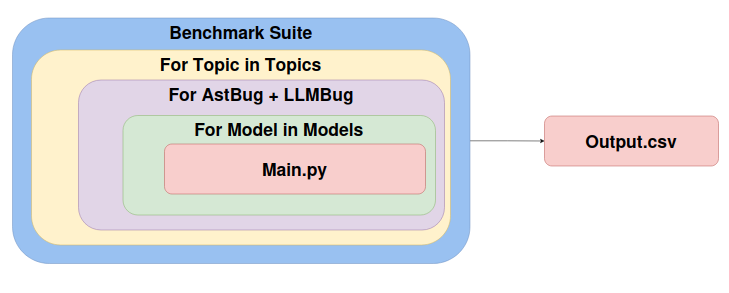
\includegraphics[width=\linewidth]{Images/Benchmark.png}

The smallest possible test is to just run the main.py file. This will simply take a default topic which was set to be the fibbonaci sequence and generate problematic code for this topic. This was the test run when implementing new features and solving the bugs that were inevitably added with the new features. This would of course be much faster than the other tests as it is only one iteration of the script being run.

The first layer on top of this is a model benchmark. This will loop through a set of models that each run the main.py script with the same parameters. This will show which model is able to create the best results and do this is an acceptable time frame. The selection of models chosen was the 32 billion parameter qwen model, the deepseek model built on top of these, the 14b parameter deepseek model, the mistral small model and the 7b llama3.1 model. The larger models were expected to perform better and slower than the smaller models. However this was not entirely consistent as will be discussed in the results section.

The second layer on top is very simple it will run the models first with abstract syntax tree bug insertion and secondly with LLM bug insertion. This will show the metrics of each method across a number of models. The results of this will be discussed in the results section.

The final layer is a loop that will run the second layer benchmark with a number of topics. This will show the metrics of each method across a number of models and a number of topics. There is little difference in the results when comparing against different topics but it is an important test to run in case some models are better at generating code for some topics than others.

\subsection{Metrics}
\subsubsection{Code Complexity}

The code complexity score is calculated using the radon python library. The cyclomatic complexity is calculated for each file using the cc visit function which takes the code in text format as an argument and will return a complexity score. The same is done for the cognitive complexity. In the output csv for each run the cognitive and cyclomatic complexity of each problem is given but for the higher layer tests only the average of the complexities is shown. The complexity score has no ideal value, it is simply an indicator of how complex or otherwise the code generated is. In some settings a high complexity may be desired while in other settings a low complexity may be desired.

\subsubsection{Code Diversity}

The code diversity score is calculated individually for each file. For each file it will compare it one by one to each of the other files, the results are then averaged to get the diversity of the file. The diversity is calculated one by one in this method because the levenstein distance function in the text distance python library only supports one to one comparison. If the diversity for a given file is below some threshold the code diversify class is used to re-prompt the LLM with the code and a prompt to create a more unique program. The diversity score itself is actually as similarity score so the lower the score of the similarity the more diverse and the better the results are.

\subsubsection{Attempt Count}

The attempt count metric is split up into two sections. There is the code generation attempt count which will give the amount of times that the LLM had to be re-prompted in order to create the code. This is generally very low and the majority of models will generate the original code with the first response most of the time. The second attempt count is the bug insertion attempt count. This is only relevant for the LLM bug insertion, it will often require 2 or 3 re-prompts of the LLM until it will produce the desired code in the correct format. This metric is important as it will indicate if a model is too simple for the task being given. The lower the attempt count is the better as it means the program was able to produce the correct results with less queries

\subsubsection{Run Time}

The run time metric is very simply the length of time it takes a given run of main.py to complete. This metric is counted in seconds as the time taken to query an LLM and for it to respond can often take 5-200 seconds with the models selected. Seconds will give the most appropriate level of detail for this metric. Of course a larger run time is bad and a lower run time is good.
\newpage
\section{Results and Discussion}

\subsection{Model Benchmark}

From the result of the model benchmark script the below graph was generate which compares the time taken, attempts taken and diversity score for each model with both LLM bug insertion and AST bug insertion.
\begin{figure}[h!]
\centering
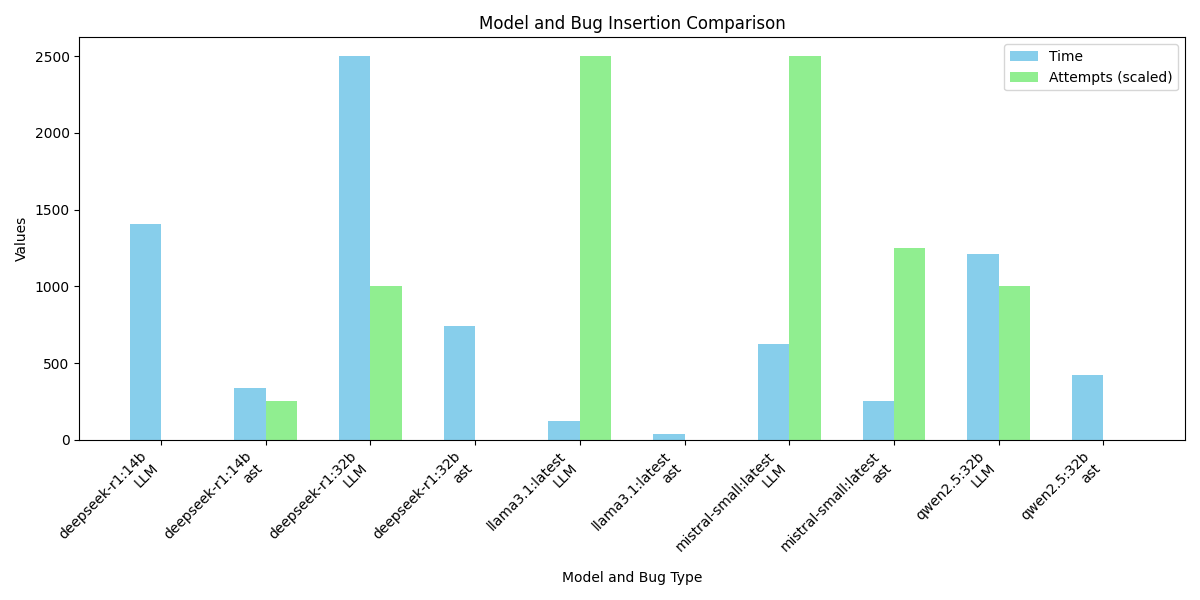
\includegraphics[width=\linewidth]{Images/Model_Comparison_Fibbonaci.png}
\label{fig:Model_Benchmark}
\end{figure}

From the graph above we see the very predictable outcome that in general the larger models will have larger runtimes. We also as expected see that the reasoning models will have substantially longer runtimes then equally sized non reasoning models. This is because the reasoning models will re-prompt a number of times over to try and improve the response as much as possible before providing a final output. The shortest runtime is from the llama3.1 model with AST bug insertion. As this is the smallest model this is expected. 

Across the board we can see a very large difference between the AST bug insertion and LLM bug insertion, for each model we can see that the runtime of the LLM bug insertion is at least two times larger, in some cases as much as four times larger. The same is seen for the attempts needed as the vast majority of the re-prompts are during the bug insertion, there is rarely a need for a retry in original code generation. We can see from this that the AST bug insertion is much more reliable and much faster than the LLM bug insertion. In the below graph we can see the metrics for cognitive complexity, cyclomatic complexity and diversity for each model which are the best indicator of the quality of the code generated.

\begin{figure}[h!]
\centering
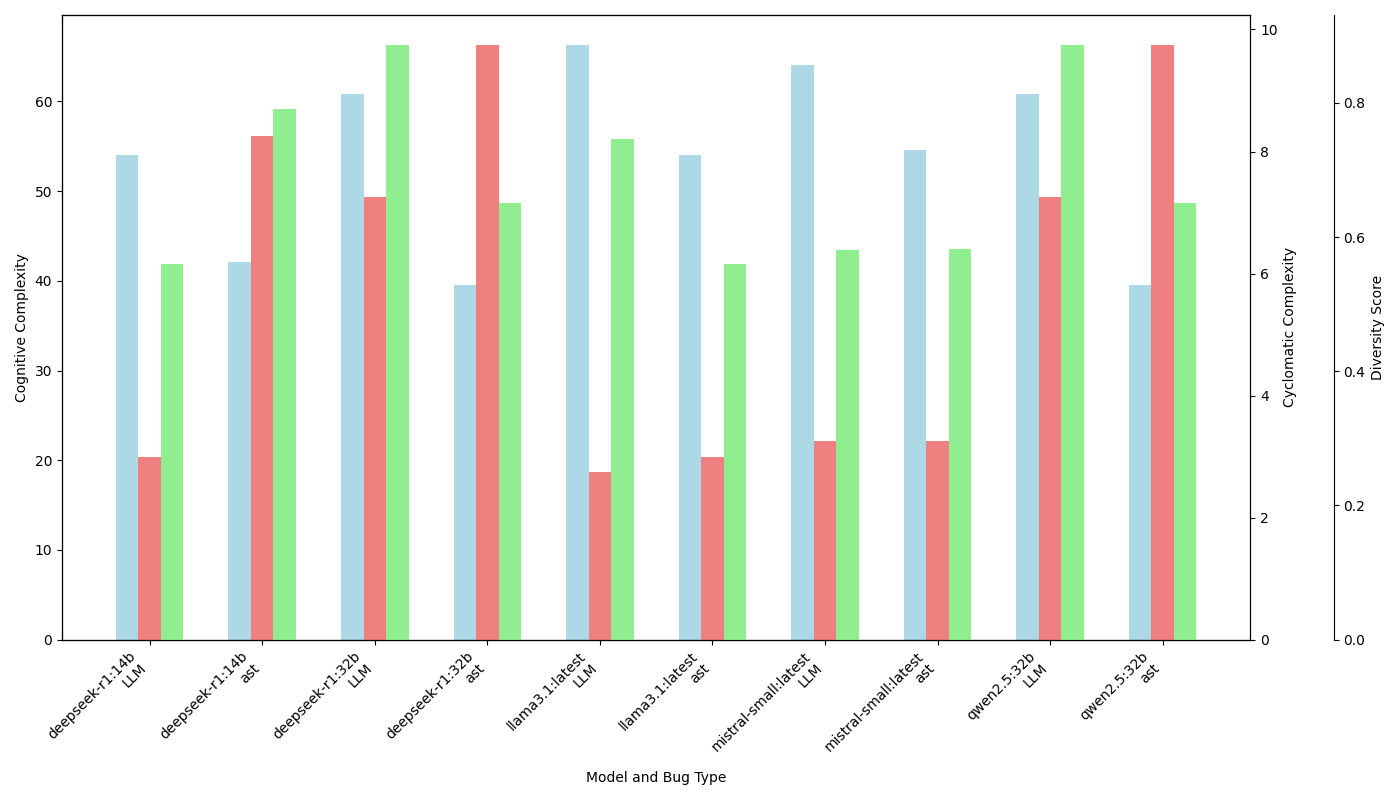
\includegraphics[width=\linewidth]{Images/Complexity_Comparison_Fibbonaci.png}
\label{fig:Complexity_Benchmark}
\end{figure}

The size of the model and the type of model has little effect on the cognitive complexity, this is because the task given to all of them was the same and there was little scope for creativity, it is possible that there would be further difference between the models with a more open ended topic which will be discussed in the next section. The cyclomatic complexity does seem to increase with the size of the model, this is likely because the larger models are generating more parameterised code that will have greater levels of nesting than the smaller models that will be more likely to generate simpler code. The diversity score also is larger with the larger models which can be attributed to the same reason as the cyclomatic complexity, the increased complexities of the code generated by the larger models will lead to a greater diversity in the code generated.

We can see that the LLM bug insertion method tends to have a higher cognitive complexity. This is likely because the bugs that it is inserting are adding more complexity to the code, whereas the AST bug insertion method is only altering working parts of the code to cause errors. The opposite result is seen for the cyclomatic complexity, this will again be because of the types of bug that are inserted. Two of the possible bug types for AST can affect the functioning of a for loop and there is also a bug type that will affect function calls which can also affect cylomatic complexity. The diversity score for both methods is quite similar,it will change from model to model which has higher diversity which is well within margin of error for the test which is not as precise as the two complexity measurements.

\subsection{Topic Benchmark}

The results of the Models with different bug insertion methods above were run for one topic. The same test was run a number more times with different topics and bug prompts. Some topics will have more or less scope for creativity and complexity which might provide an interesting comparison between the bug insertion methods under different circumstances.

The first topic that was tested was Arrays. This is a very simple topic which tests how the models and methods performed with a more constrained topic.

\begin{figure}[h!]
\centering
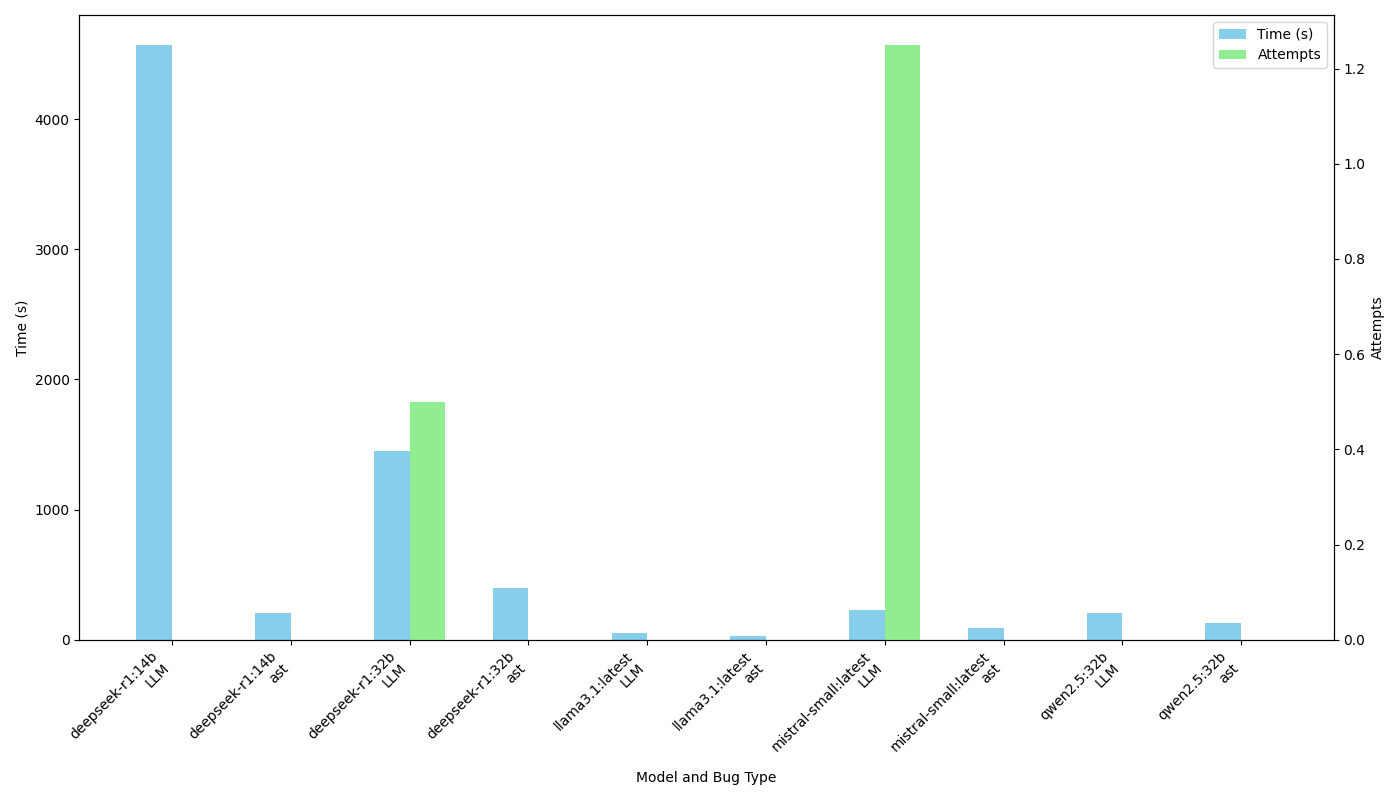
\includegraphics[width=0.8\linewidth]{Images/Model_Comparison_Arrays.png}
\caption{Model Comparison Arrays}
\label{fig:Model_Comparison_Arrays}
\end{figure}

\begin{figure}[h!]
\centering
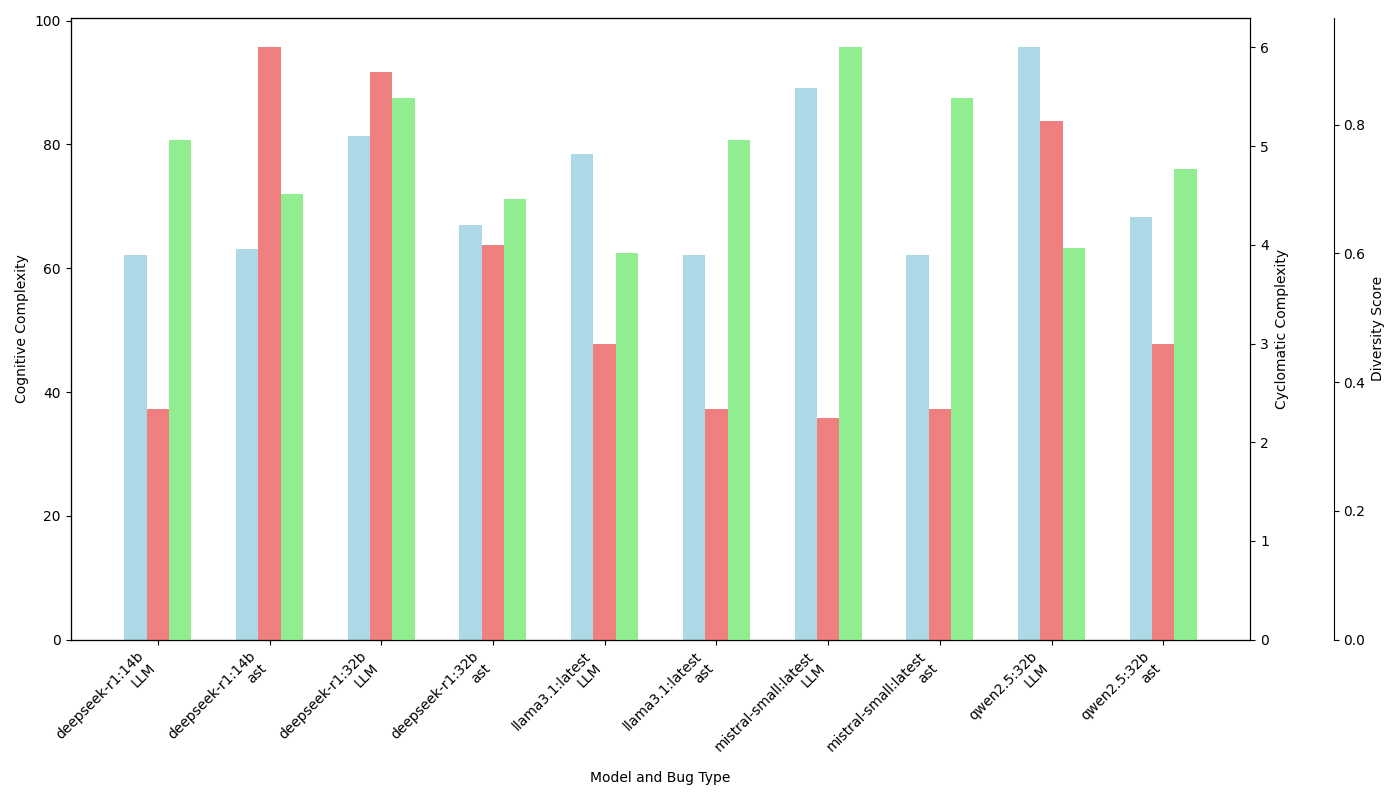
\includegraphics[width=0.8\linewidth]{Images/Complexity_Comparison_Arrays.png}
\caption{Complexity Comparison Arrays}
\label{fig:Complexity_Comparison_Arrays}
\end{figure}

The results of both graphs in this case are very similar to that of the baseline. They follow the exact same trend but the scale is different. The results of the array topic take longer to generate, take more retries and provide more complex code, the diversity however is not improved from the baseline.

The next topic that was tested was the Djikstra algorithm. From the broad phrasing of the topic we can expect to see more meaningful results in this case.

\begin{figure}[h!]
\centering
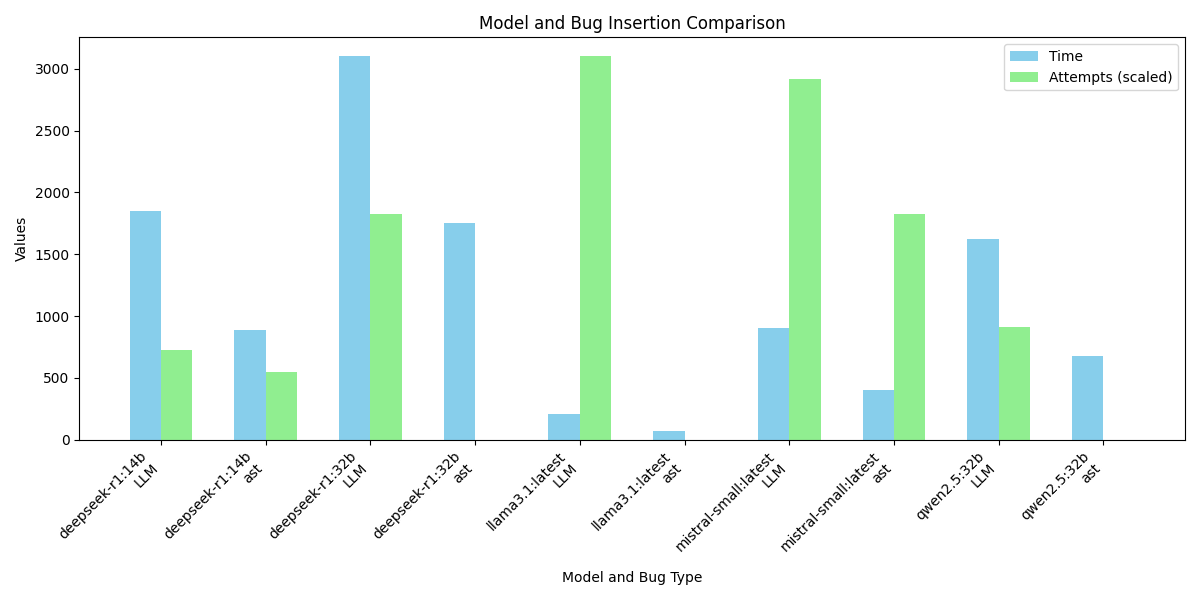
\includegraphics[width=0.8\linewidth]{Images/Model_Comparison_Djikstra.png}
\caption{Model Comparison Djikstra}
\label{fig:Model_Comparison_Djikstra}
\end{figure}

\begin{figure}[h!]
\centering
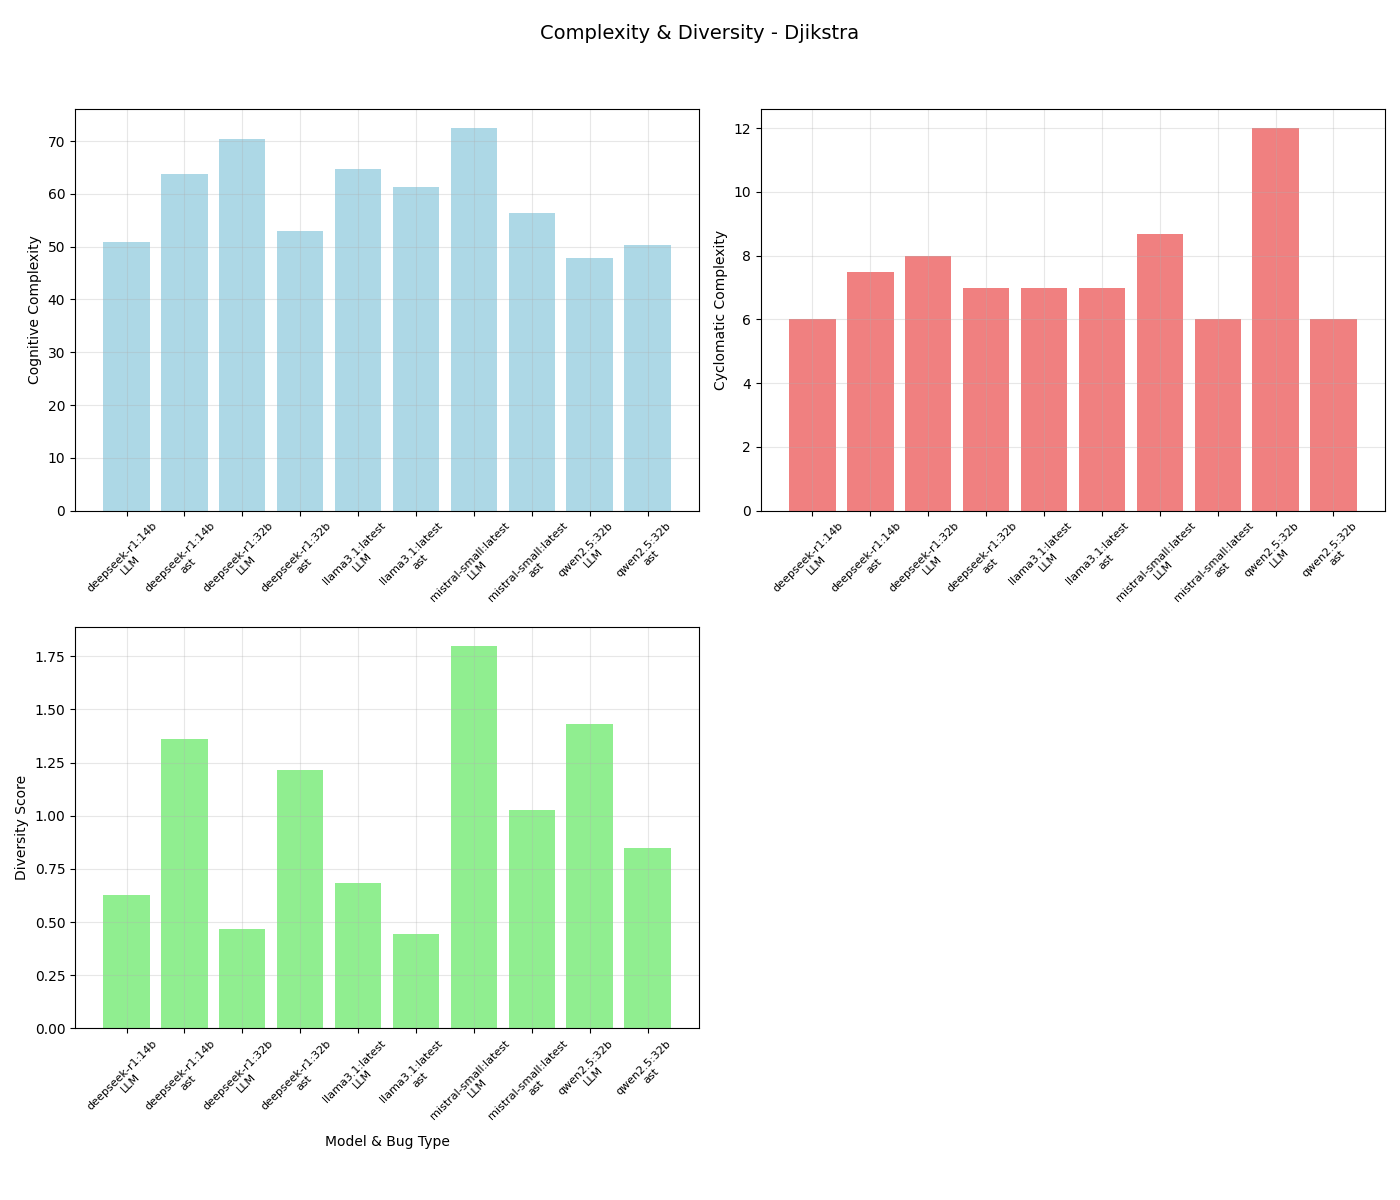
\includegraphics[width=0.8\linewidth]{Images/Complexity_Comparison_Djikstra.png}
\caption{Complexity Comparison Djikstra}
\label{fig:Complexity_Comparison_Djikstra}
\end{figure}

Much like above these graphs too follow the same trend across models but the scale is different again. There runtime and attempts required are both much higher than the baseline. this is due to the task being more complex, this is clearly only the case in the LLM bug insertion as there is no increase in attempts for the AST bug insertion, from this we can take that the LLM bug insertion becomes much less feasible for larger more complex code while the AST bug insertion will perform consistently in any setting. From the second graph we also see the expected increase in complexity and diversity from the baseline.

\begin{figure}[h!]
\centering
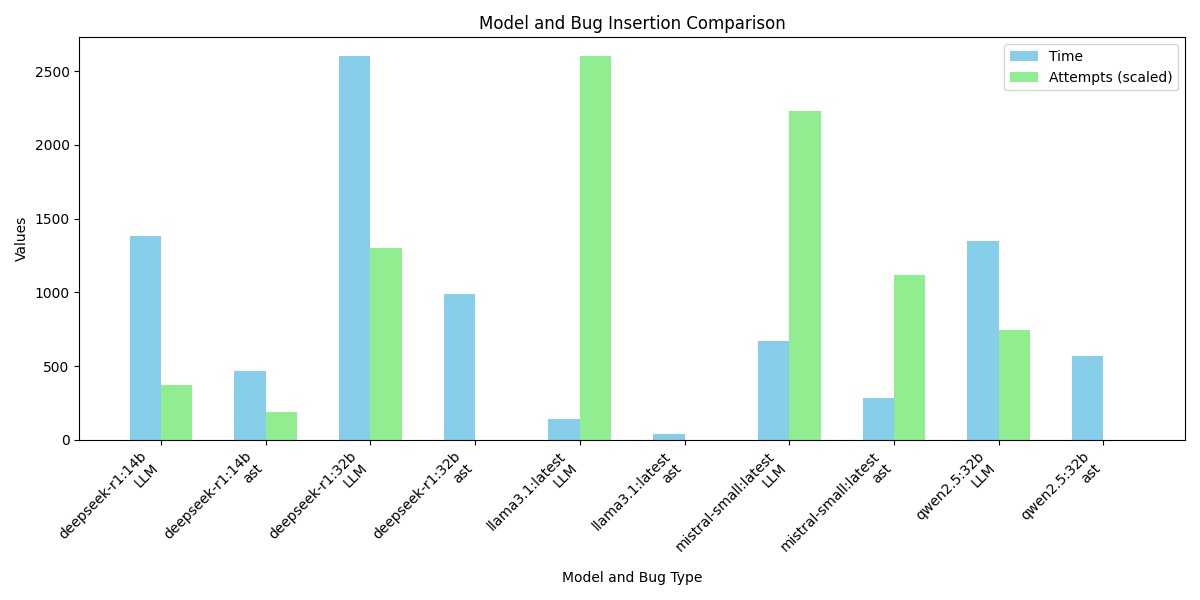
\includegraphics[width=0.8\linewidth]{Images/Model_Comparison_Linked_Lists.png}
\caption{Model Comparison Linked Lists}
\label{fig:Model_Comparison_Linked_Lists}
\end{figure}

\begin{figure}[h!]
\centering
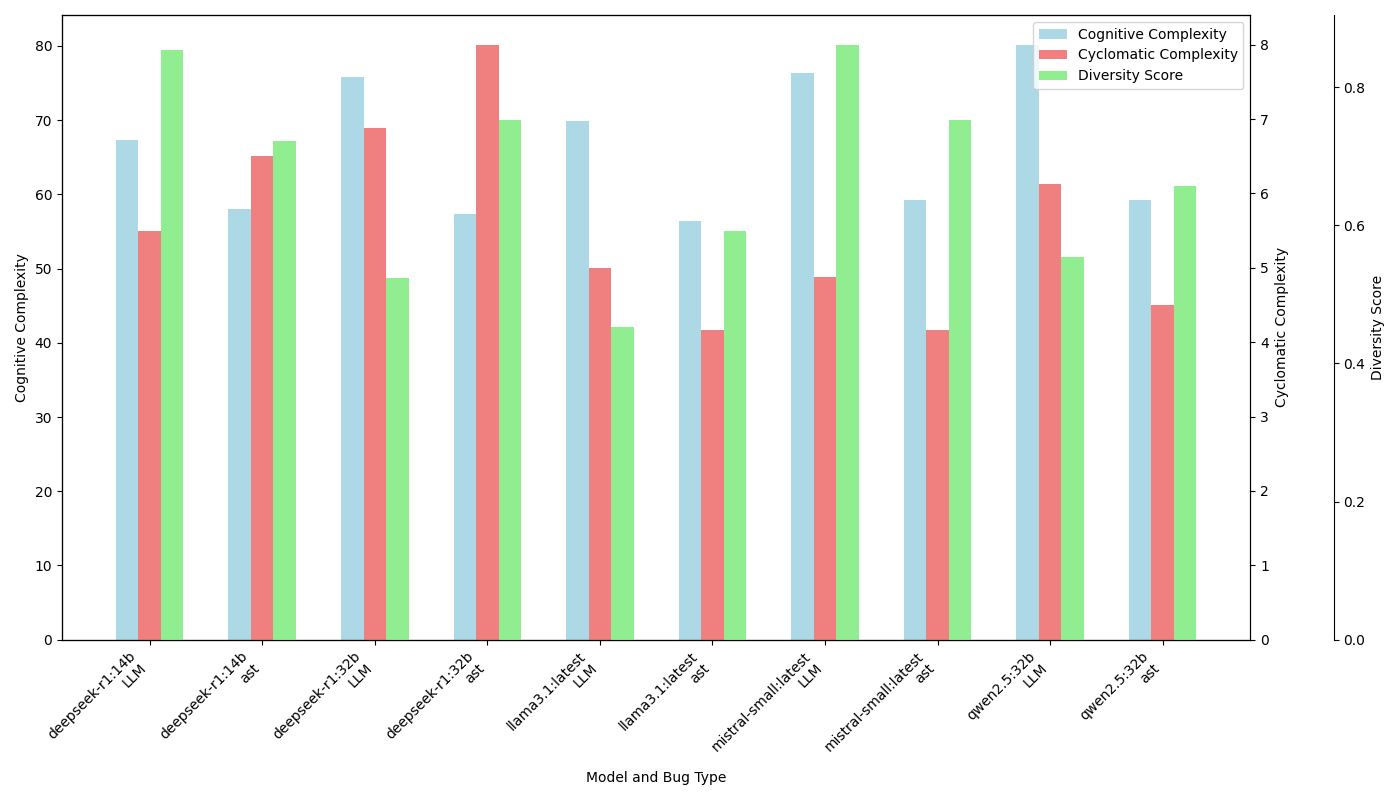
\includegraphics[width=0.8\linewidth]{Images/Complexity_Comparison_Linked_Lists.png}
\caption{Complexity Comparison Linked Lists}
\label{fig:Complexity_Comparison_Linked_Lists}
\end{figure}

The linked lists topic had performance between the baseline and the djikstra topic. The runtime and attempts required were comfortably higher than the baseline but not quite as high as djikstra, particularly for the attempts required. The complexity and diversity scores were very similar to the baseline and were not increased significantly. 

\begin{figure}[h!]
\centering
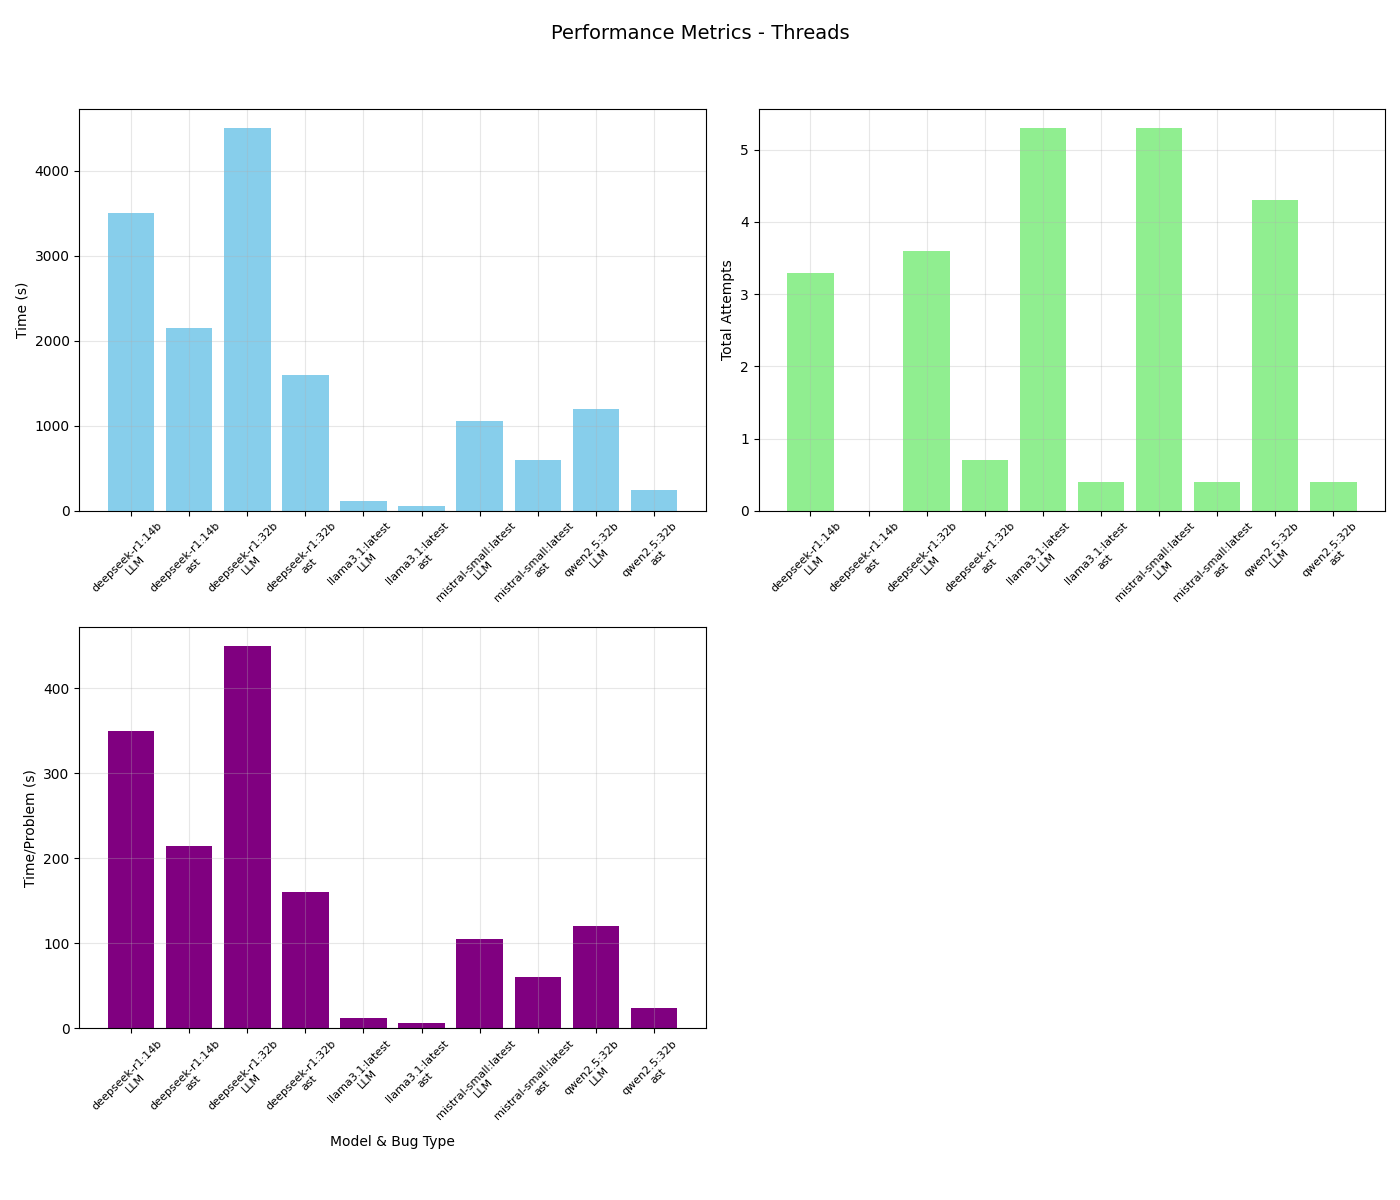
\includegraphics[width=0.8\linewidth]{Images/Model_Comparison_Threads.png}
\caption{Model Comparison Threads}
\label{fig:Model_Comparison_Threads}
\end{figure}

\begin{figure}[h!]
\centering
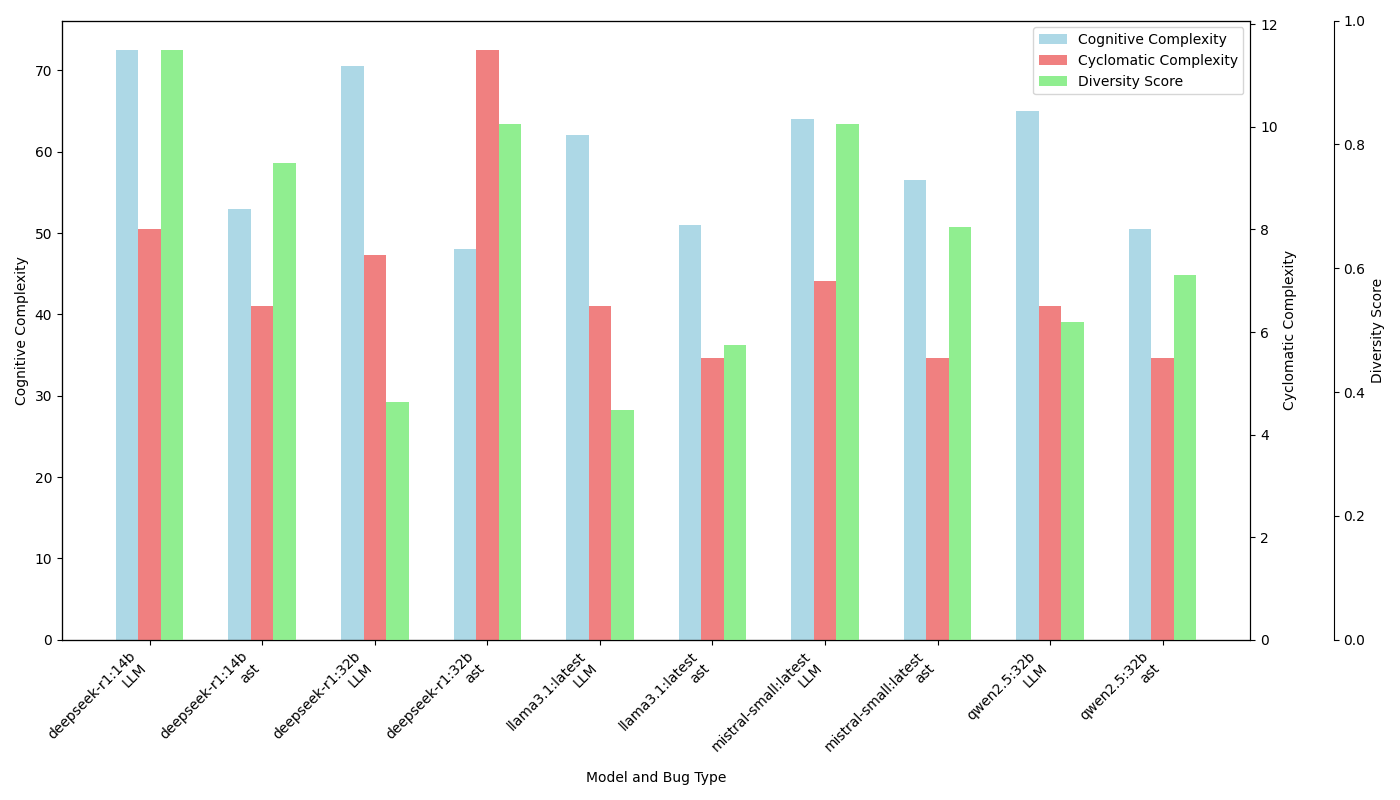
\includegraphics[width=0.8\linewidth]{Images/Complexity_Comparison_Threads.png}
\caption{Complexity Comparison Threads}
\label{fig:Complexity_Comparison_Threads}
\end{figure}

The multi-threading topic had very similar results to djikstra as both have high levels of nesting and subsequent complexity. However where it does differ is the diversity score, the multi-threading does not see nearly as diverse results as djikstra. Examing the output code this appears to be because each case of multi-threading defaulted to the same few fundamental examples of a deadlock while the djikstra topic had no clear bug to insert and so the results were much more varied.

\subsection{Hyperparameter Tuning}

From all of the above testing a lot of data for model performance was collected. There has been no testing for the optimal hyperparameters for these models though. This will only be done for the best performing model in the previous examples. There is clear best model but considering the trade off between run time, reliability (attempts needed) and diversity the qwen2.5:32b model gives reliable, high quality results and does not take too excessive a quantity of time like the deepseek models. For that reason the hyperparameter-tuning will be performed on the qwen2.5:32b model using AST bug insertion. The parameters that will be tuned are the temperature, the max tokens, the top p and the top k. The temperature controls the amount of randomness in the output, the max tokens controls the maximum length of the output, the top p controls the probability of the output token being selected and the top k controls the number of tokens that are considered for the output. The tuning will be done using a grid search approach where the model will be run with a large set of possible combination of hyperparameters and the results will be compared. 


\newpage
\section{Conclusion}

This will briefly summarise the project and discuss the future of the project.

\newpage
\section{References}
\begin{thebibliography}{9}

\bibitem{jadud2006}
Jadud, M. C. (2006). Methods and tools for exploring novice compilation behaviour. Proceedings of the Second International Workshop on Computing Education Research, 73–84. https://doi.org/10.1145/1151588.1151600

\bibitem{li2019}
Li, C., Chan, E., Denny, P., Luxton-Reilly, A., \& Tempero, E. (2019). Towards a Framework for Teaching Debugging. Proceedings of the Twenty-First Australasian Computing Education Conference, 79–86. https://doi.org/10.1145/3286960.3286970

\bibitem{odell2017}
O’Dell, D. H. (2017). The Debugging Mindset: Understanding the psychology of learning strategies leads to effective problem-solving skills. Queue, 15(1), 71–90. https://doi.org/10.1145/3055301.3068754

\bibitem{parkinson2024}
Parkinson, M. M., Hermans, S., Gijbels, D., \& Dinsmore, D. L. (2024). Exploring debugging processes and regulation strategies during collaborative coding tasks among elementary and secondary students. Computer Science Education, 0(0), 1–28. https://doi.org/10.1080/08993408.2024.2305026

\bibitem{whalley2021}
Whalley, J., Settle, A., \& Luxton-Reilly, A. (2021). Analysis of a Process for Introductory Debugging. Proceedings of the 23rd Australasian Computing Education Conference, 11–20. https://doi.org/10.1145/3441636.3442300

\bibitem{whalley2023}
Whalley, J., Settle, A., \& Luxton-Reilly, A. (2023). A Think-Aloud Study of Novice Debugging. ACM Transactions on Computing Education, 23(2), 1–38. https://doi.org/10.1145/3589004

\bibitem{denny2023}
Denny, P., Leinonen, J., Prather, J., Luxton-Reilly, A., Amarouche, T., Becker, B. A., \& Reeves, B. N. (2023). Promptly: Using Prompt Problems to Teach Learners How to Effectively Utilize AI Code Generators. https://doi.org/10.48550/ARXIV.2307.16364

\bibitem{denny2024}
Denny, P., Leinonen, J., Prather, J., Luxton-Reilly, A., Amarouche, T., Becker, B. A., \& Reeves, B. N. (2024). Prompt Problems: A New Programming Exercise for the Generative AI Era. Proceedings of the 55th ACM Technical Symposium on Computer Science Education V. 1, 296–302. https://doi.org/10.1145/3626252.3630909

\bibitem{nguyen2024}
Nguyen, S., Babe, H. M., Zi, Y., Guha, A., Anderson, C. J., \& Feldman, M. Q. (2024). How Beginning Programmers and Code LLMs (Mis)read Each Other. Proceedings of the CHI Conference on Human Factors in Computing Systems, 1–26. https://doi.org/10.1145/3613904.3642706

\end{thebibliography}

\end{document}